% ==================================
%
% PFC FRANCISCO SANCHEZ ARROYO
%
%===================================

\documentclass[a4paper,12pt,titlepage]{article}
\usepackage[includehead,includefoot]{geometry}
\geometry{left=2.5cm,right=2.5cm,top=2cm,bottom=2cm}
\usepackage{graphicx}
\usepackage[utf8]{inputenc} % Caracteres con acentos. 
\usepackage{longtable}
%\usepackage[spanish]{babel}
\usepackage{latexsym}
\usepackage{fancyhdr}
\usepackage{amsmath}
\usepackage{tabulary}
\usepackage{amssymb}
\usepackage{rotating} %rotar tablas y mas
\usepackage{hyperref}
\usepackage{lscape}
% Poner colorlinks=false para la version impresa
\hypersetup{colorlinks=false, linkcolor=red,citecolor=green,filecolor=magenta,urlcolor=cyan}
%\usepackage{eurosym}
\usepackage{titlepic} %imagenes en la portada
\usepackage{lettrine}
\usepackage{booktabs} \usepackage{tabulary} %Para ajustar anchos de tablas
%% Cambia el formato de las cabeceras de las tablas y figuras
%\usepackage[small,normal,bf,up]{caption2}
%\renewcommand{\captionfont}{\small\itshape}
\usepackage{verbatim}
\usepackage{smartdiagram}
\usesmartdiagramlibrary{additions} 
\usepackage{tikz}
\usetikzlibrary{shapes}
%\usepackage[active,tightpage,floats]{preview}
%\setlength\PreviewBorder{5pt}%

%\titlepic{\includegraphics[width=12cm]{storefront.pdf}}
\title{Fabricating Labs\\
\Huge \textbf{Guidelines for designing and planning Fab Labs, Makerspaces and Innovation Facilities}}
\author{
by Francisco Sanchez Arroyo\\
The (Fabulous) Beach Lab
}
\date{Barcelona. \today}

%=====================================================
%=====================================================
\begin{document}

%\renewcommand{\tablename}{Taula}
%\renewcommand{\figurename}{Figura}
%\renewcommand{\listtablename}{Index de Taules}

% Values for plots
\newcommand{\D}{6} % number of dimensions (config option)
\newcommand{\U}{5} % number of scale units (config option)

\newdimen\R % maximal diagram radius (config option)
\R=3.5cm 
\newdimen\L % radius to put dimension labels (config option)
\L=4.3cm
% end values for plots


\newcommand{\A}{360/\D} % calculated angle between dimension axes  

\maketitle

\tableofcontents % Tabla de contenido
\clearpage
%\pagenumbering{roman}


%\addtocontents{toc}{\hfill Page \endgraf}
%\addtocontents{toc}{\bfseries Agradecimientos\endgraf}%
%\newpage
%\listoffigures % Índice de figuras
%\newpage 
%\listoftables % Índice de tablas 
%\newpage

\pagenumbering{arabic}



% Estilo de Cabecera y pie de pagina
\pagestyle{fancy}
\rhead{\textit{\textbf{Fabricating Labs}}}
\lhead{\textit{Guidelines for designing and planning Innovation Spaces}}
\cfoot{-Page \thepage -}

\section*{About the author}
My name is Francisco Sanchez Arroyo, I am a MSc.Civil Engineer with specialty in Structural Engineering by the Polytechnic University of Catalonia. I am also an accredited LEED AP in Building Design and Construction by the GBCI. I graduated in Fab Academy and Bio Academy programs by The Academy of (Almost) Anything.\\ 

In late 2012, I decided to quit my job in Real Estate Property Developement and focus in the maker movement and stablishing my own innovation space, The Beach Lab. I am passionate about education, technology, innovation and the environment, I balance my borderless citizenship with the love of my 2 wonderful sons.\\

Please feel free to reach me with any questions or comments about any of these topics.\\

\noindent{\url{hola@beachlab.org}}\\
\noindent{\url{http://beachlab.org}}\\
\noindent{\url{https://www.linkedin.com/in/fsancheza}}

\section*{License}
This work is licensed under Creative Commons Attribution ShareAlike 4.0 International License (CC BY-SA 4.0). 

\section*{Disclaimer}
This guide is permanent work in progress, check the build date at the cover page. It might also contain errors and omisions. Handle with care.
\clearpage
\section{Introduction}
Are you planning to set up a Fab Lab or Makerspace? The most common mistake is starting with the machines and then figuring out the rest later. But did you think about why do you want these machines? What are the challenges that you want to solve with them?  What about the technical and operational aspects? Did you consider the workflows around each machine? Are the other uses inside a room compatible with the new process?  What about the sustainability aspects of building design and construction? How will you foster a respectful workplace? This Guide is intended to help you identifying all the factors involved, cover the basic requirements and to avoid generating future problems related to inadequate planning.\\

As a member of a global network of interconnected labs, I have had the opportunity to
visit, set up, fix and operate many fab labs around the world, including mine, The Beach Lab. I not
only help fab labs to streamline the setup, operation and training of their facilities. I also
guide them to create better spaces that are not just rooms with a bunch of equipment, but
promote the development of a strong sharing community and interaction of its members.\\

While this document will need to be further
developed, it will settle the foundations for the work to be elaborated in your planning process.

\section{The Strategic Plan}
\textit{- I want a Fab Lab}\\ 
- Cool. Why?\\ 
\textit{- I don't know, everybody has one, and we need to have one too}\\ 

I agree, you probably need to have one too. But if you don't know why, and what is the challenge that you want to solve, and then allocate the resources to make it happen, it will not happen. Because a bunch of machines in a room is not magic. No matter how big you make it, no matter how many machines you fit inside, no matter how advanced is the technology. It will not happen.\\ 

What is a Fab Lab or makerspace or an innovation space anyway? Think about it. It's not the machines, it's the people, the right kind of people. You will be using the facility to attract, gather and empower people. Because if you keep thinking that when you buy the machines you are done, you are right: It's over. Innovation requires a different mindset, open minded leadership. The most important change of this movement is the disruptive opportunity where tiny actors -that are free to move and fail very fast- can compete globally with rigid established giants in equal conditions, peer-to-peer.\\  

The strategic plan of the lab is a fundamental document in the foundation of the initiative and must give answer to why do you want it, what is the particular challenge and the most important, what is the vision in a mid/long term. Where do you want to be next year or five years from now? Because you need a path to follow. Not only for the future operation, but also for the planning and construction. 

\section{The Planning Process}
Planning and executing a Fab Lab requires to complete some linear phases that cannot be executed in parallel. But you can --and should-- revisit and iterate on them when something does not work. The fastest, the better.
\begin{description}
\item[Phase 0:] Develop the strategic plan of the lab. Identify your mid and long term goals, your challenges and your environment. Sign it and stick to it. But as I said before, these are not the 10 commandments. You can change them if they don't work.
\item [Phase 1:] According to the above, list the capabilities you would need to have in the Fab Lab. Elaborate your inventory according to your budget. This is a important step because you don't want to end up with duplicated equipment, missing equipment/materials, materials of doubtful utility and unbalanced number of machines.

\item [Phase 2:] Analyze the needs of these machines and their hosting spaces in terms of MEP (Mechanical, electrical,plumbing) and HSE (health, safety and environment). Determine which are the rooms that are
more suitable for each type of machine.
\item [Phase 3:] Determine a layout plan for the separation of the spaces.
\item [Phase 4:] Elaborate a plan to implement furniture, MEP and HSE needs.
\item [Phase 5:] Develop and execute the chosen solution.
\item [Phase 6:] Establish a respectful and healthy work environment. Plan the activities. Welcome users.
\end{description}

This guide will not cover phases zero and one. Not that I don't want to, but this is the essence of the initiative, its soul and unique DNA fingerprint that will define the entity and requires a personalized answer.   

\section{What is the Ideal Layout?}
\subsection{Short answer} 
No such thing.

\subsection{Long answer}
There is not and ideal layout for a Fab Lab. Some people will tell you it's the \textit{Chicago Layout}\footnote{\url{http://fabfoundation.org/index.php/ideal-lab-layout/index.html}}, the only problem is that you are not probably in Chicago or have a space like them. Every fab lab has its owns singularities that make
them unique spaces. What makes all Fab Labs so great orbits around a very simple idea that
is represented in the three men holding each one shoulder in Fab Lab logo. \textit{Fab Labs are
places to learn, to make and to share}. And these three basic concepts, should have a physical representation in the layout. 

\begin{figure}[ht] %  figure placement: here, top, bottom
   \centering
   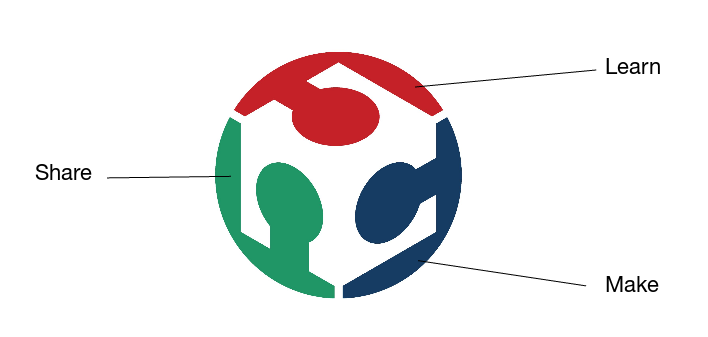
\includegraphics[width=8cm]{files/learn-make-share} 
\end{figure}


\subsection{Principles and Values to foster}
What you should focus instead is in \textit{impact}. Good Labs make impact, so that they engage more users to participate and be part of the collaborative movement. There are some key values that we must try to embed into the fab lab:

\begin{description}
\item[Sustainability.] This is a key and fundamental concept that it's behind the origin of fab labs itself. Our planet is our legacy. Remember, there is no plan(et) B. LEED design guidelines (specially Building Design + construction) can help in the design and contruction of a sustainable and environmentally respectful space.
\item[Flexibility.] The space should serve many purposes. A flexible design can virtually multiply
the space in your lab, making it suitable for many different activities. You can plan ahead of time and try to predict the future. But a more intelligent approach is designing resiliency. Allowing change to happen and be less traumatic. Examples are furniture and machines on wheels, incorporating hanging power cords, open
ceilings and flexible ducts for lasers exhausts.
\item[Modularity.] The space should be able to grow or shrink as the needs of the lab progresses.
\item[Sharing and collaboration.] The spaces we create should encourage people to cooperate together. That means furniture that do not separate people, spaces that do not separate people, and environments acd activities that require cooperative solutions.
\item[Sand Box.] The lab is a fail safe environment for experimentation. If everything is so shiny, so clean, so beatiful that cannot be disturbed without loosing this beauty, then nothing will happen inside.
\end{description}

If you want to send a powerful message, you must show and transmit these values through every
aspect in the fab lab, from the activities happening inside, to the layout, to the furniture you have, to the
materials you use and to the spirit of the staff.

\begin{figure}[h] %  figure placement: here, top, bottom
   \centering
   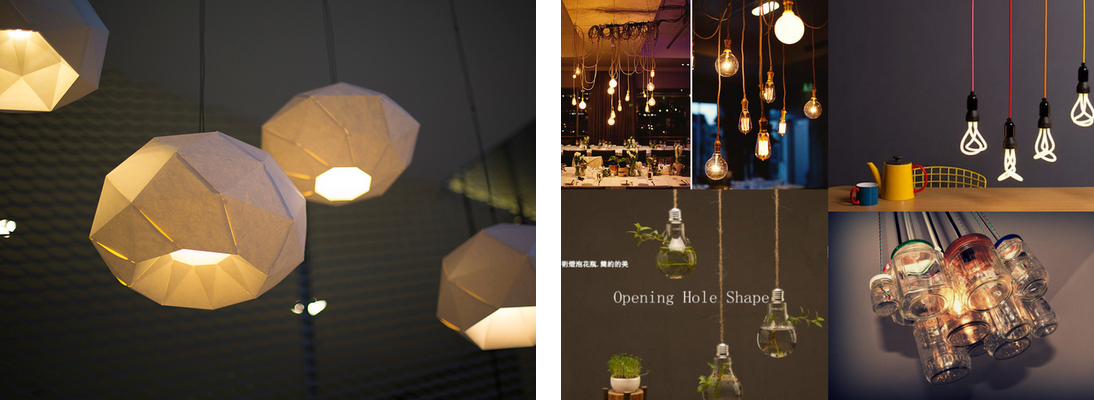
\includegraphics[width=16cm]{files/lamps} 
   \caption{Lamps fabricated using tools in the lab as lasercutters and upcycled materials.}
\end{figure}

\begin{figure}[h] %  figure placement: here, top, bottom
   \centering
   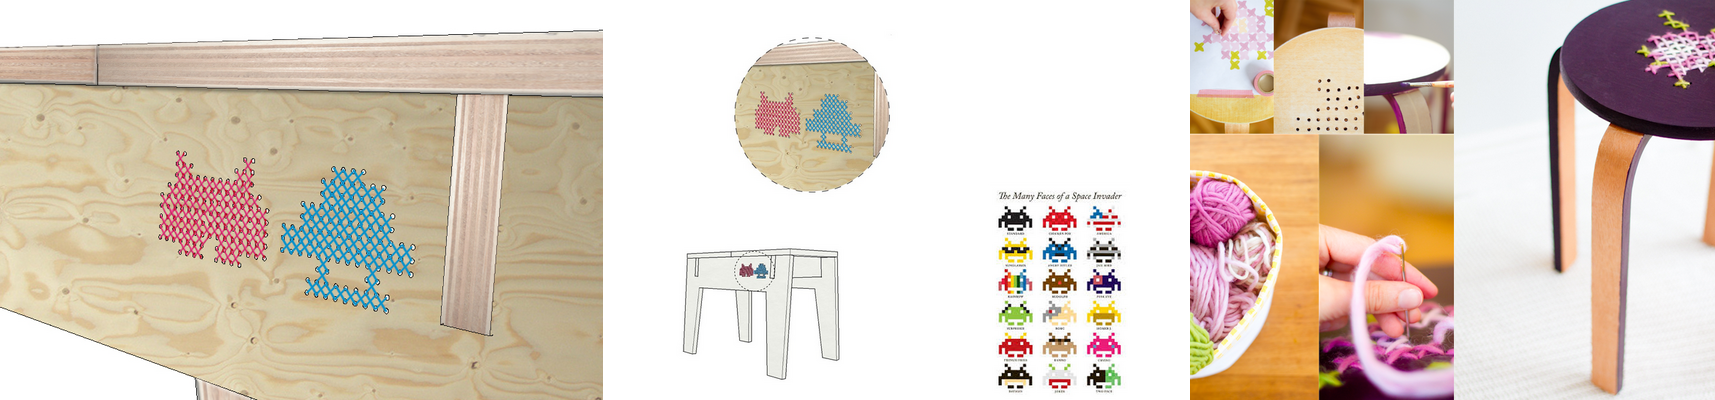
\includegraphics[width=16cm]{files/knit} 
   \caption{Existing furniture can be hacked to promote customization and collaborative designs.}
\end{figure}

\begin{figure}[h] %  figure placement: here, top, bottom
   \centering
   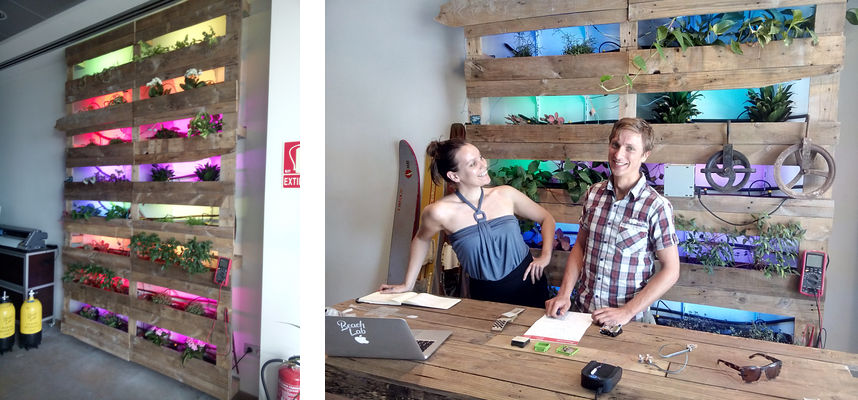
\includegraphics[width=16cm]{files/pallet} 
   \caption{Pallet wood can be used to create amazing furniture and related workshops. In this
picture \textit{The Beach Lab} in Spain, showing a table and a vertical garden with embedded
electronics that displays the amount of water in the soil using color codes.}
\end{figure}

\clearpage
\section{Learning, making, sharing}
\subsection{The Sharing Space}
The sharing space could be considered as a sort of mixer. It is, by far, the
most important of the 3 spaces
found in fab labs. If we fail to
have a sharing space there will
not be a community to build
around. Ideally it is an open-access, informal space where
people meet and gather
together and interact. In most
places it builds around food
and drink, adopting the form of
a maker cafe, or a shared
kitchen. This space is suitable
for all kind of interactions, and
to showcase projects. And it is
a relaxed environment for new
members of the lab, who can
enter and see what is
happening inside the lab in a
format that is friendly and
known to them. We should
avoid formalisms as corporate
receptions which will not help
in this kind of spaces.

\begin{figure}[h] %  figure placement: here, top, bottom
   \centering
   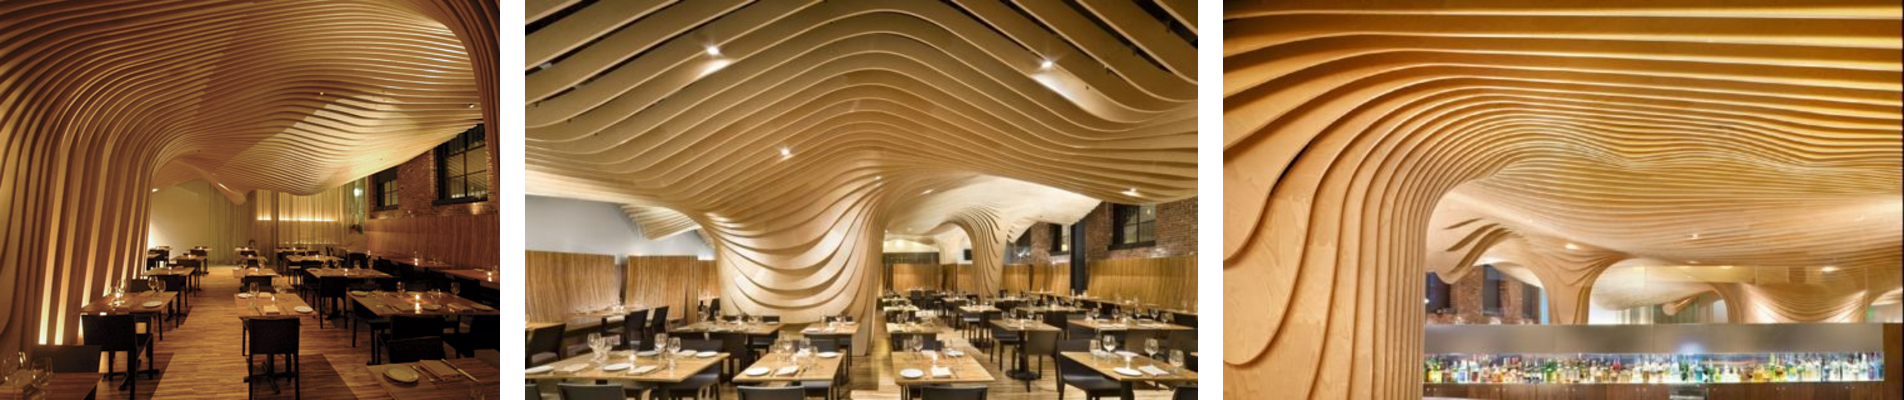
\includegraphics[width=16cm]{files/roof} 
   \caption{Natural renewable materials like wood should be prioritized in the design of the fab lab.
In this picture, a Shopbot machine has been used to design a custom organic shapes. In
this kind of lab fabricated environments, it is easy to engage conversations and to
explain the values of prototyping, design and collaborative assembly.}
\end{figure}

\begin{figure}[h] %  figure placement: here, top, bottom
   \centering
   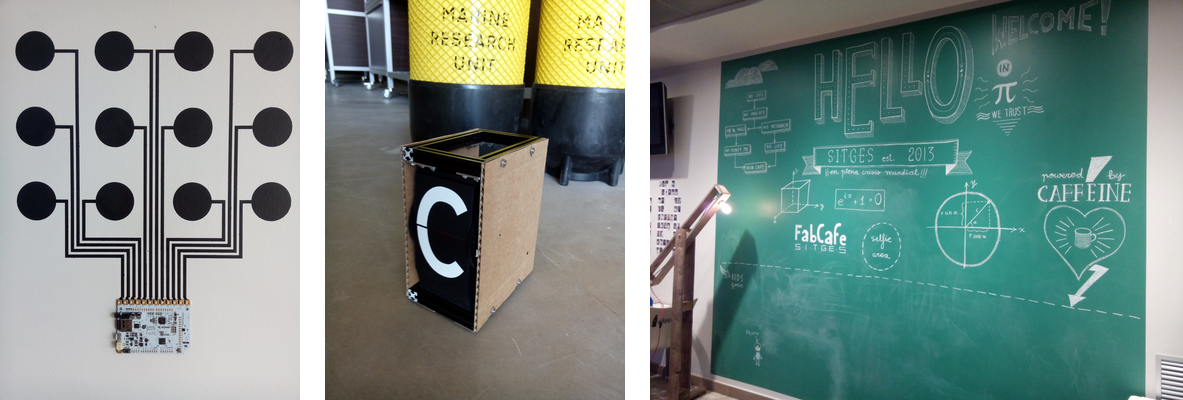
\includegraphics[width=16cm]{files/sharing2} 
   \caption{The sharing space is a great space to display projects developed in the fab lab. In this
picture \textit{The Beach Lab}. On the left a custom control panel for the lights of the fab lab.
In the center a split flap display to display twitter messages. On the right a collaborative
chalkboard where people can express their creativity. Some other spaces also have
some kind of collaborative walls with lego parts that the members keep filling up. Or white sculptures that people draw with markers.}
\end{figure}

\begin{itemize}
\item Ideal place to gather around drink and eat (kitchen)
\item Soft seating
\item Displays Showing: 
\begin{itemize}
\item dashboards (visitors, key performance indicators)
\item Calendar with upcoming workshops and events
\end{itemize}
\item Tablets for visitors self registration system
\item Mini houses
\item Photocall
\item Phone booths
\item Area for showcasing projects
\item Interactive wall
\item Creativity wall
\end{itemize}

\subsection{The Learning Space}
The design of the
Learning Space can be
envisioned as hybrid
classroom/lab.
This flexible
classlab blend
elements of traditional
classroom and
laboratories to
support the students working
in several disciplines
(biology, mechanics,
electronics, etc.) at the same time. Students in these spaces typically work in
groups of three, collaborating on real world science problems.\\ 

If space allows, it is recommended to dedicate a big central space as auditorium, where all the members can gather to attend
lectures, guest speakers and perform big presentations and announcements. Otherwise, the Sharing Space is where this public activities also fit well.

%\item[Learning by doing.]


\subsection{The Making Space}
The Making Space is the kernel of the fab lab, it's \textit{where things happen}. This
space  usually host incompatible uses that make mandatory a division of the making space into 2 areas. The clean and quiet, and the loud and messy. If you can afford it you could organize the 2 areas around \textit{The
Assembler}, which is a central area with multipurpose tables to assemble and work in projects.
The Assembler needs to be very versatile to be able to host very diverse projects, in terms of
people participating and space and resources required. In this main area you could also have specificic shared design resources like a library of books/reading corner, multimedia production hardware for the creation and edition of audio and video content, VR technologies and 3D mouse for increased CAD productivity.\\

\begin{figure}[h]
\centering
\smartdiagram[bubble diagram]{The\\ Assembler, Loud and\\ Messy, Quiet and\\ Clean}
\end{figure}
The Making Space is where you want to start thinking about access-control. It's not about forbidding or restricting users. It's about  knowing who enters and whether they have the proper credentials and safety knowledge to operate the equipment. Because this is the area of the fab lab where potentially dangerous equipment is.

\subsubsection{The clean and quiet}

\subsubsection{The loud and messy} 


\subsection{Outdoors}
\begin{itemize}
\item Events
\item Interviews
\item Showcasing
\item Chillout Bars
\item Farm/greenhouse
\item Pavilions and structures
\item Natural environment: Forest/desert/beach/sea/lakes/rivers
\end{itemize}

\clearpage  
\section{Processes and Workflows}

\subsection{Aspects to be assessed}
\begin{description}
\item [Operational Logistics:] How will the assets and people flow in, out and around? How will you manage the inventory (including maintenance, storage and locking requirements)? How will you control access? What's the maintenance plan? Is the facility ready for redundancy and resiliency when some equipment fail?

\item [Mechanical, Electrical and Plumbing (MEP) requirements:] Under this category it is included lighting requirements, HVAC systems, piping and plumbing, power and electrical requirements. Paying special attention to using the natural resources (natural lighting, natural ventilation, etc.) that can lower the environmental footprint of the facility.

\item [Health, Safety and Environment (HSE):] We should take very seriously Health, Safety and Environment aspects in Fab Labs. It's our social responsibility and our legacy to take care of the users, faculty and employees.
The inventory of equipment, materials, workflows and processes that Fab Labs use and recommend have been
carefully selected in order to comply with the highest standards of HSE. This also includes ergonomy and waste management.
\end{description}

\subsection{Levels of assessment}
When planning a Fab Lab, the above elements should be assessed in 4 levels of detail:
\begin{itemize}
\item \textbf{The machine or process}. Each machine and process has its owns requirements.
\item \textbf{The workflow around that machine or process}. A machine it's usually part of a bigger process or workflow, whose requirements you need to analyse too. If workflows
are not identified, machines and materials will be  placed randomly (incorrectly) placed without a
logical arrangement. Ideally every machine and process should follow a logic workflow and
have all its materials, inflows and outflows at reaching distance.

\item \textbf{The room containing that workflow} must be analysed specially looking for incompatibilities regarding noise, dust, ventilation, etc. Not only Learning, making and sharing spaces should be separated. Within the making
area of the lab, there should be separation of clean and quiet with loud and messy areas to avoid incompatible uses colliding.
\item \textbf{The building containing that room} must be assessed as well. High frecuency vibrations created by digital fabrication machines can travel through the structure of the building causing trouble in areas very far areas from its origin.
\end{itemize}



% Please add the following required packages to your document preamble:
% \usepackage{booktabs}
% \usepackage{lscape}
\begin{landscape}
\subsection{Summary of processes}
\begin{table}[h]
\centering
\begin{tabular}{@{}lllllllll@{}}
\toprule
Process                & Messy & Dust & Water & Noise       & Lighting & Access Lock & Temp & Ventilation \\ \midrule
3D Printing FDM        & No    & No   & No    & Moderate    & No       & No          & Yes           & Yes \\
3D Printing Resin      & Yes   & No   & No    & Low         & No       & No          & No            & Yes         \\
Laser Cutting          & No    & No   & No    & Medium/High & No       & No          & No            & Yes         \\
CNC                    & Yes   & Yes  & No    & High        & No       & Yes         & No            & Yes         \\
Electronics Production & No    & Yes  & Yes   & Moderate    & Yes      & No          & No            & Yes         \\
Vinyl Cutting          & No    & No   & No    & Low         & Yes      & No          & No            & No          \\
Industrial Robot Arm   & Yes   & Yes  & Yes   & Medium/High & No       & Yes         & No            & Yes         \\
Bio Lab                & Yes   & No   & Yes   & Low         & Yes      & Yes         & Yes           & Yes         \\
Sewing Machines        & No    & No   & No    & Low         & Yes      & No          & No            & No          \\
Molding and Casting    & Yes   & No   & Yes   & Moderate    & No       & No          & No            & Yes         \\ \bottomrule
\end{tabular}
\caption{Table of processes}
\label{processes}
\end{table}
\end{landscape}

\subsection{Vinyl Cutting}
\begin{figure}[h]

\centering
\smartdiagramset{
    set color list={red!10, red!25,red!40, red!55},
    sequence item border color=black,
    sequence item text color=black,
    sequence item border size=1.2\pgflinewidth,
    sequence item font size=\scriptsize\sffamily,
    additions={
        additional item shape=rectangle,
        additional item fill color=gray!20,
        additional item border color=black,
        additional arrow line width=2pt,
        additional arrow tip=to,
        additional arrow color=black,
        additional item font=\scriptsize\sffamily,
      }
}
\smartdiagramadd[sequence diagram]{Materials (1),Machine (2) \\ Roland GX 24, Postprocess\\ (3), Waste (4)}
{below of sequence-item1/{Raw and scrap material},below of sequence-item2/Reusable Scrap}
\smartdiagramconnect{to-}{sequence-item1/additional-module1}
\smartdiagramconnect{-to}{sequence-item2/additional-module2}
\vspace{1cm}
\end{figure}
\subsubsection*{Notes}
\begin{itemize}
\item (1) Additional items: X-acto, scissors, masking tape, vinyl gloves
\item (2) This area requires also space for a computer for design and operation tasks. Provide enough power plugs (minimum 3)
\item (2) The back of the machine must be reachable
\item (2) Additional items: Tweezers, X-acto, scissors
\item (3) This area requires the witdh of the biggest roll that the machine can handle and plenty of light
\item (3) Additional items: Tweezers, X-acto, scissors
\item (4) Waste: Paper backing, vinyl, Copper film, epoxy film.
\end{itemize}
\subsubsection*{Risks}
\begin{itemize}
\item Hand trapped by machine movement
\item Cuts with sharp objects
\end{itemize}
\subsubsection*{Personal Protective Elements (PPE)}
\begin{itemize}
\item None required
\end{itemize}
\clearpage

\subsection{3D Printing FDS}
\begin{figure}[h]

\centering
\smartdiagramset{
    set color list={red!10, red!25,red!40, red!55},
    sequence item border color=black,
    sequence item text color=black,
    sequence item border size=1.2\pgflinewidth,
    sequence item font size=\scriptsize\sffamily,
    additions={
        additional item shape=rectangle,
        additional item fill color=gray!20,
        additional item border color=black,
        additional arrow line width=2pt,
        additional arrow tip=to,
        additional arrow color=black,
        additional item font=\scriptsize\sffamily,
      }
}
\smartdiagramadd[sequence diagram]{Materials (1),Machine (2) \\ 3D printer, Postprocess\\ (3), Waste (4)}
{below of sequence-item1/Filament}
\smartdiagramconnect{to-}{sequence-item1/additional-module1}
\vspace{1cm}
\end{figure}
\subsubsection*{Notes}
\begin{itemize}
\item (1) Filaments require low moisture environment
\item (3) Additional items: Wire cutter, spatula
\item (2) Machine requires rear inspection
\item (2) Power requirements: Most 3D printers don't require a computer. Newest require network connection.
\item (2) HVAC direct airflow or low room temperature might affect buildplate adhesion and layer cooling
\item (3) Additional items: X-acto, pliers, wire cutter
\item (4) PLA and ABS based plastics
\end{itemize}
\subsubsection*{Risks}
\begin{itemize}
\item Hand trapped by machine movement
\item Burn by noozle or buildplate
\item Hot plastic splatters caused by moisture inside filament
\end{itemize}
\subsubsection*{Personal Protective Elements (PPE)}
\begin{itemize}
\item Eye protection is recommended for kids
\end{itemize}
\clearpage

\subsection{3D Printing SLA}


\subsection{Laser Cutting}
\begin{figure}[h]

\centering
\smartdiagramset{
    set color list={red!10, red!25,red!40, red!55},
    sequence item border color=black,
    sequence item text color=black,
    sequence item border size=1.2\pgflinewidth,
    sequence item font size=\scriptsize\sffamily,
    additions={
        additional item shape=rectangle,
        additional item fill color=gray!20,
        additional item border color=black,
        additional arrow line width=2pt,
        additional arrow tip=to,
        additional arrow color=black,
        additional item font=\scriptsize\sffamily,
      }
}
\smartdiagramadd[sequence diagram]{Materials (1),Machine (2) \\ Laser Cutter, Postprocess\\ (3), Waste (4)}
{below of sequence-item1/{Raw and scrap material},below of sequence-item2/Reusable Scrap}
\smartdiagramconnect{to-}{sequence-item1/additional-module1}
\smartdiagramconnect{-to}{sequence-item2/additional-module2}
\vspace{1cm}
\end{figure}
\vspace{0.3cm}
Laser is usually operating full time and it is also noisy enough to disturb any learning activities. Another problem to foresee is the fumes of the laser. Even you have a filter, when you enter the room there is going to be noticeable smell. In part because people will not respect the exhaust times before opening the lid and in part because the filter is not perfect. Hence the room requires air renovation from the exterior.

\subsubsection*{Notes}
\begin{itemize}
\item (1) Maintaining order of scrap material is important
\item (1) Cardboard and wood are sensitive to moisture
\item (2) The room requires ventilation and air renovation from exterior
\item (2) The laser is usually a noisy environment, specially if there is also a filter installed
\item (2) It is required also space for computer for design and operation of the laser
\item (2) Power requirements: Provide at least 6 power plugs
\item (3) Clean up scrap material and store it in (1)
\item (4) Cardboard, wood, plastics
\end{itemize}
\subsubsection*{Risks}
\begin{itemize}
\item Health issues due to long-term exposure to fumes 
\item Cuts by sharp edges of material
\end{itemize}
\subsubsection*{Personal Protective Elements (PPE)}
\begin{itemize}
\item Recommended gloves for handling material and scrap
\end{itemize}

\clearpage


\subsection{Electronics Production}
\begin{figure}[h]
\centering
\smartdiagramset{
    set color list={red!10, red!25,red!40, red!55, red!70},
    sequence item border color=black,
    sequence item text color=black,
    sequence item border size=1.2\pgflinewidth,
    sequence item font size=\scriptsize\sffamily,
    additions={
        additional item shape=rectangle,
        additional item fill color=gray!20,
        additional item border color=black,
        additional arrow line width=2pt,
        additional arrow tip=to,
        additional arrow color=black,
        additional item font=\scriptsize\sffamily,
      }
}
\smartdiagramadd[sequence diagram]{Design (1),Machine (2) \\ SRM 20, Stuff (3), Test (4),Waste (5)}
{below of sequence-item2/{FR1 boards and milling bits},below of sequence-item3/Electronic components}
\smartdiagramconnect{to-}{sequence-item2/additional-module1}
\smartdiagramconnect{to-}{sequence-item3/additional-module2}
\vspace{1cm}
\end{figure}
\subsubsection*{Notes}
\begin{itemize}
\item (1) Area for a computer next to the machine for design and machine operation. 3 power plugs
\item (2) Additional items: Spatula, double-side tape, X-acto, Allen keys for milling bits, magnets
\item (3) As this usually becomes a bottleneck of the process a minimum of 2 seats for soldering operators should be plannned
\item (3) Easily accessible cabinets with electronic components
\item (3) This area requires ventilation and air renovation, plenty of light and magnifying equipment
\item (3) Power requirements for 2 seats: 6 plugs
\item (4) 2 seats area for power supply, oscilloscope and function generator. Power requirements 6 plugs
\item (5) Waste: Paper dust, FR1 boards, broken bits, electronic components
\end{itemize}
\subsubsection*{Risks}
\begin{itemize}
\item Fumes inhalation
\item Electric shock
\item Cuts by sharp objects
\item Burns by soldering iron
\end{itemize}
\subsubsection*{Personal Protective Elements (PPE)}
\begin{itemize}
\item Gloves for removing boards and soldering
\item Eye protection for soldering
\item Isolating shoes
\end{itemize}
\clearpage


\subsection{Molding and Casting}
Molding and casting is a 3-phase process that can be done at different time and in separated rooms
\begin{figure}[h]

\centering
\smartdiagramset{
    set color list={red!10, red!25,red!40, red!55},
    sequence item border color=black,
    sequence item text color=black,
    sequence item border size=1.2\pgflinewidth,
    sequence item font size=\scriptsize\sffamily,
    additions={
        additional item shape=rectangle,
        additional item fill color=gray!20,
        additional item border color=black,
        additional arrow line width=2pt,
        additional arrow tip=to,
        additional arrow color=black,
        additional item font=\scriptsize\sffamily,
      }
}
\smartdiagramadd[sequence diagram]{Materials (1),Machine (2) \\ SRM 20}
{below of sequence-item1/{Machinable wax},below of sequence-item2/Reusable Wax chips}
\smartdiagramconnect{to-}{sequence-item1/additional-module1}
\smartdiagramconnect{-to}{sequence-item2/additional-module2}
\vspace{1cm}
\end{figure}

\begin{figure}[h]

\centering
\smartdiagramset{
    set color list={green!10, green!25,green!40},
    sequence item border color=black,
    sequence item text color=black,
    sequence item border size=1.2\pgflinewidth,
    sequence item font size=\scriptsize\sffamily,
    additions={
        additional item shape=rectangle,
        additional item fill color=gray!20,
        additional item border color=black,
        additional arrow line width=2pt,
        additional arrow tip=to,
        additional arrow color=black,
        additional item font=\scriptsize\sffamily,
      }
}
\smartdiagramadd[sequence diagram]{Preprocess (3),Molding (4), Waste (5)}
{below of sequence-item1/{Silicons and Rubbers},below of sequence-item2/Reusable Soft Mold}
\smartdiagramconnect{to-}{sequence-item1/additional-module1}
\smartdiagramconnect{-to}{sequence-item2/additional-module2}
\vspace{1cm}
\end{figure}

\begin{figure}[h]

\centering
\smartdiagramset{
    set color list={yellow!10, yellow!25,yellow!40},
    sequence item border color=black,
    sequence item text color=black,
    sequence item border size=1.2\pgflinewidth,
    sequence item font size=\scriptsize\sffamily,
    additions={
        additional item shape=rectangle,
        additional item fill color=gray!20,
        additional item border color=black,
        additional arrow line width=2pt,
        additional arrow tip=to,
        additional arrow color=black,
        additional item font=\scriptsize\sffamily,
      }
}
\smartdiagramadd[sequence diagram]{Preprocess (6),Casting (7), Waste (8)}
{below of sequence-item1/{Casting Materials}}
\smartdiagramconnect{to-}{sequence-item1/additional-module1}
\vspace{1cm}
\end{figure}

\subsubsection*{Notes}
\begin{itemize}
\item (1)(2) Phase 1 can be executed in the same room as electronics production. But it requires to clean and vacuum the machine and surrounding area prior to milling the wax. This phase produces virtually zero waste. A dedicated vacuum machine or a clean brush is recommended to pick up all the wax chips for future use.
\item Phase 2 and Phase 3 can be executed in a separate room. These phases require a ventilated area and access to water and a sink.
\item (3) Refer to MSDS for important health and safety information
\item (4) Store reusable molds in the same storage room as silicons
\item (5) Waste: Pots, gloves, sticks, etc, stained with silicons and rubbers
\item (8) Waste: Pots, gloves, sticks, etc, stained with casting materials
\end{itemize}
\subsubsection*{Risks}
\begin{itemize}
\item Inhalation of dangerous volatile substances
\item Eye, skin and lung irritation
\end{itemize}
\subsubsection*{Personal Protective Elements (PPE)}
\begin{itemize}
\item Lab coat, vinyl gloves and eye protection during the molding and casting phases
\item Masks and respirators upon the MSDS specs of the materials
\end{itemize}
\clearpage


\subsection{Composites}
Composites is a 2-phase process that can be done at different time and in separated rooms
\begin{figure}[h]

\centering
\smartdiagramset{
    set color list={red!10, red!25,red!40, red!55},
    sequence item border color=black,
    sequence item text color=black,
    sequence item border size=1.2\pgflinewidth,
    sequence item font size=\scriptsize\sffamily,
    additions={
        additional item shape=rectangle,
        additional item fill color=gray!20,
        additional item border color=black,
        additional arrow line width=2pt,
        additional arrow tip=to,
        additional arrow color=black,
        additional item font=\scriptsize\sffamily,
      }
}
\smartdiagramadd[sequence diagram]{Materials (1),Machine (2) \\ Shopbot, Waste (3)}
{below of sequence-item1/{High Density Foam}}
\smartdiagramconnect{to-}{sequence-item1/additional-module1}
\vspace{1cm}
\end{figure}

\begin{figure}[h]

\centering
\smartdiagramset{
    set color list={green!10, green!25,green!40},
    sequence item border color=black,
    sequence item text color=black,
    sequence item border size=1.2\pgflinewidth,
    sequence item font size=\scriptsize\sffamily,
    additions={
        additional item shape=rectangle,
        additional item fill color=gray!20,
        additional item border color=black,
        additional arrow line width=2pt,
        additional arrow tip=to,
        additional arrow color=black,
        additional item font=\scriptsize\sffamily,
      }
}
\smartdiagramadd[sequence diagram]{Preprocess (4),Composite Layout (5), Waste (6)}
{below of sequence-item1/{Fabrics and Resins},below of sequence-item2/Reusable Mold}
\smartdiagramconnect{to-}{sequence-item1/additional-module1}
\smartdiagramconnect{-to}{sequence-item2/additional-module2}
\vspace{1cm}
\end{figure}


\subsubsection*{Notes}
\begin{itemize}
\item (2) Room containing the Shopbot is a very noisy, dusty and dangerous environment. Recommended separate room.
\item (2) Room containing the Shopbot must have ventilation and filtration system. Refer to calculations in following sections.
\item (3) Waste: Foam dust, high density foam
\item (4) This phase requires a ventilated area and access to water and a sink
\item (5) Store reusable molds in (1)
\item (6) Waste: Sand paper and resin dust
\end{itemize}
\subsubsection*{Risks}
\begin{itemize}
\item Fine dust particles inhalation in milling phase
\item Fast spinning cutting tool in milling phase
\item Debris in milling phase
\item Noise damage
\item Being trapped by moving machine or spindle
\item Eye, skin and lung irritation due to resins
\end{itemize}
\subsubsection*{Personal Protective Elements (PPE)}
\begin{itemize}
\item Eye, ear protection
\item Appropriate gloves for handling materials
\item Coat, eye protection, gloves and mask/respirators during composite layout phase
\end{itemize}
\clearpage


\subsection{Large CNC}
\begin{figure}[h]

\centering
\smartdiagramset{
    set color list={red!10, red!25,red!40, red!55},
    sequence item border color=black,
    sequence item text color=black,
    sequence item border size=1.2\pgflinewidth,
    sequence item font size=\scriptsize\sffamily,
    additions={
        additional item shape=rectangle,
        additional item fill color=gray!20,
        additional item border color=black,
        additional arrow line width=2pt,
        additional arrow tip=to,
        additional arrow color=black,
        additional item font=\scriptsize\sffamily,
      }
}
\smartdiagramadd[sequence diagram]{Materials (1),Machine (2) \\ Shopbot, Waste (3)}
{below of sequence-item1/{Wood}}
\smartdiagramconnect{to-}{sequence-item1/additional-module1}
\vspace{1cm}
\end{figure}
\subsubsection*{Notes}
\begin{itemize}
\item (1)(3) You need to think about the materials inflow/outflow and storage for this room.
\item (2) The room containing the Shopbot is a very noisy, dusty and dangerous environment. Recommended separate room.
\item (2) The room containing the Shopbot must have ventilation and filtration system. Refer to specs below.
\item (2) This room is appropriate for woodwork machinery, sandblasting, compressor and metalworking.
\item (2) This room might require soundproofing. The bad news about acoustic isolation is that it works like waterproofing. Doesn't matter how well you isolate everything, if you leave a weak area, the sound will scape through that weak spot. That is to say: If you are not thinking of properly isolating don't waste your time and money. 
\end{itemize}

\subsubsection*{Risks}
\begin{itemize}
\item Fine dust particles inhalation in milling phase
\item Very sharp milling bits
\item Fast spinning cutting tool\footnote{Extreme caution with long hair, visitor cards, and anything hanging from your body and tied to it.}
\item Debris in milling phase
\item Being trapped by moving machine
\end{itemize}
\subsubsection*{Personal Protective Elements (PPE)}
\begin{itemize}
\item Eye, ear protection
\item Appropriate gloves for handling materials and milling bits
\end{itemize}

\subsubsection*{Filtration System}
Most of the time you are going to be working with wood materials. This equipment
produces a loud and dusty environment. So, the first advice is
placing all this equipment in a separated room. Most of these machines come with
a dust collector that will capture the thicker wood particles. But still there will be finer cloud
particles up to 10 micron that will not only float for around 30 minutes, but also will be
suspended again with the slightest movement of air. The fine dust becomes a serious health issue. These
fine particles will come from 2 sources. One is the dust collection felt bag that will allow
particles up to 3 microns to escape through the fabric. And the second source is particles that because their high speed will never enter the dust collection system.\\

So I suggest that you install in these rooms a filtration system rated so that it will cycle through
the entire volume of air in the room 6 to 8 times per hour. And with a timer for 2, 4, or 8 hours
so that when the user will walk out of the room will flip the switch and forget about it.

\subsubsection*{Avoiding dust leaving the room}
You can avoid dust exiting the CNC room by keeping the room underpressurized. That way you ensure that if there is airflow, it will be inwards. A simple way to achieve this effect is pumping out (filtered) air to any interior space adjacent to the CNC room.

\section{Using the Lab to build the Lab}
Labs do not require a lot of furniture. Most of the machines you will install are self standing. You can fabricate your own furniture with the equipment that you are installing in your lab rather than buying it. That includes, not only chairs, desks and cabinets, but also lamps, security equipment, access control, surveillance and alarms, upcycling old machines or furniture you find on the street and giving them a new life, etc. That way you will not only be showing machines in those general public visits, but also show actual things that you have made with them. Giving meaning to the investment that you made and credit to the people who worked on them. So my recommendation is do not buy anything new, use temporary or old things that you already have, and make a plan for building your own stuff. You can even create workshops around this self-fabrication process that will start gathering a community with a strong sense of belonging and pride of the facility. Great examples are FAB13 conference, The Green Lab, Soko Lab, The Beach Lab and many others.

\subsection{\textit{Made in a Fab Lab} brand}

\subsection{Making your own Furniture}

\subsubsection{Using someone else's designs}

\url{http://opendesk.cc} is a well known place with plenty of designs ready to mill and assemble. You will require some materials.
\begin{itemize}
\item MDF boards. Not for milling the furniture. You need at least two for the sacrificial layer of the Shopbot. If the price difference its not too big, ask for the one with no added formaldehydes.
\item Plywood boards. Check the unit cost and origin (China, Malaysia, etc.). You can estimate around 20 full size boards for a complete fab lab furniture set.
\item OSB boards. This is cheaper and bad quality. But still good for certain uses.
\end{itemize}

\subsubsection{Creating your own designs}
You can also design your own variants of flat furniture. Always test first a scale model with cardboard and lasercutter. Another option is tensioned furniture and structures. All you require are bearings for fabricating pulleys and hemp/jute rope.\\

Consider any kind of local wood (dead palms, dead palm leaves, dry branches) for furniture or decoration. We have to think of using local resources before importing fresh wood.

\subsubsection{Pallets}
Shipping pallets and ideal for quickly building furniture while you reuse and upcycle existing wood. If they are old/used/broken better. Marked as HT, DB or MB only (debarked). You maybe get them for free. Once you find a good source you will need to get a Jagsaw, presurized water to clean them and a set of different length (20mm-80mm) wood screws.

\subsubsection{Giving old furniture a second life}
Old wooden furniture (not particle boards), even broken, for upcycling or bringing back to life

\subsection{Other fabricatable items}
You might need to visit car-scrapping shops, flea markets in search some treasures. Also keep all junk electronics (old computers, radios, televisions, printers...) for sourcing electronic components, mechanical components, difficult to find screws, power supplies, etc.
\begin{itemize}
\item Lamps: 3D printed and lasercut lamps. All you need is plugs, lamp cord and lamp switches.
\item Alarm, CCTV systems, access control. There are many open source projects in the Internet.
\end{itemize}
\subsection{Giving the space modularity and flexibility}
Something thar worked very well in The Beach Lab is was put all the machines on wheeled furniture. That way you could move a 3D printer, or the precission milling machine or even the vinyl cutter from one room to another when it was required or quickly move them and store them for events. This mobility will virtually increase the size of your lab as you will have much more versatility. All you need is Casters (wheels) for the furniture, whith yokes which are rubber wheeled surface.\\

Hanging AC power outlets. Consider having tables with full integrated electric and lighting subsystem and connect the table to the ceiling using spring electrical cable.

\section{Becoming a Super Lab}
At some point your lab might naturally jump to the next level and provide the community with a unique space
that becomes an international reference. In the network we call it a Super Fab Lab. A
Super Fab Lab it's not just a lab with increased capabilities in terms of space and
machinery. It is also attached to leaders with  deep values and vision, there is much more planning and strategy involved and it is something that
cannot be done in one go. You will need to correct and change things as the
community reacts. Will your lab become one of the
leading labs in the world, the ones that you can enumerate with just one hand, on par
with labs of the level of Barcelona, Amsterdam and Boston? Let's see if you have what it takes.
\subsection{The Champion}
No half-measures here. Either you have it or not. As stated in Fab Foundation page, the Champion is a fundamental human resource for the success of the
venture. It is someone who has the Fab Lab values, the passion for the job and a visionary goal for
the future. If he/she is not within the founder team of the space, bad news ahead. It might take some time to find your Champion, or it might never show up. They might
come from the faculty, students or members. My advice is to try to identify \textit{The One} within your community. If it
ever shows up, make sure you empower him to lead and drive the lab to the next level.

\subsection{Team Diversity}
One of the surprising things about fab labs is that the most beautiful and meaningful projects are never created by engineers. Engineers are weird people, and I can talk first hand here, while fundamental for their technical and organizational skills, need to be complemented by other kind of people. I
recommend that you incorporate a broader set of people, skilled in arts, design and
architecture to better attract, serve and guide the community in their projects. 


\section{Going Wireless, the Mobile Lab}
It might be helpful at this point describing the different points of view behind the concept \textit{mobile fab lab}:

\begin{itemize}
  \item Some people might understand a mobile fab lab as a movable version of the fixed space. Hence, an entire room with wheels. I won't cover this vision in this chapter. You will need a truck/bus big enough as a room to lay/secure your equipment as we usually do in fixed spaces.
  \item Some other envision it as a pop-up lab. This requires a reduced/incomplete subset of the equipment enclosed in movable, deployable furniture. Usually used for demo purposes.
  \item I consider a mobile lab as an iteration of the fixed space, an evolution pursuing a reduction of space through combination of capabilities. The lab happens to be embedded in a vehicle, but could be fitted in a desktop, instead of occupying an entire room. This requires deep changes in the selection of the machinery, tools, energy sources, waste management, storage and so on.
\end{itemize}




\section{What's next?}

Engaging the community.



\end{document}
